\documentclass[]{report}
\usepackage{graphicx}
\usepackage{geometry}
\usepackage{amssymb}
\usepackage{textcomp}
 \geometry{
 a4paper,
 total={170mm,257mm},
 left=20mm,
 top=20mm,
 width=17cm,
 }
\usepackage{ragged2e}

\begin{document}
\begin{center}
 {\Large Data Intensive Computing - Review Questions 4}
\end{center}
\begin{center}
 {\small Daniele Montesi, Francesco Staccone}
\end{center}
\vspace{1cm}
\justify
\begin{enumerate}
 \item What is DStream data structure, and explain how a stateless operator, such as map, works on DStream?\\
 
 A Discretized Stream (DStream), the basic abstraction in Spark Streaming, is a continuous sequence of RDDs (of the same type) representing a continuous stream of data. DStreams can either be created from live data (such as, data from HDFS, Kafka or Flume) or can be generated by transformation existing DStreams using operations such as map, window and reduceByKeyAndWindow. While a Spark Streaming program is running, each DStream periodically generates a RDD, either from live data or by transforming the RDD generated by a parent DStream.\\
 A stateless operator, such as the map(\textit{func}), returns a new DStream by passing each element of the source DStream through a function \textit{func}.
 
 \item Explain briefly how mapWithState works, and how it differs from updataStateByKey.\\
 
 Spark Streaming is able to handle state-based operations, complex event processing problems that are based on storing some current state and updating it based on incoming events in subsequent batches of data. Spark API proposes two function to do that:\\
 \begin{itemize}
 \item \textit{ mapWithState}, that is executed only on set of keys that are available in the last micro batch. As result performance is proportional to the size of the batch;\\
 \item \textit{updateStateByKey}, that is executed on the whole range of keys in DStream. As results performance of these operation is proportional to the size of the state.\\
 \end{itemize}
 They both are executed on PairDStream (JavaPairDStreaml) and require checkpoints activation.\\
 More in detail about the improvements introduced by mapWithState:\\
 -at every batch arrival, updateStateByKey iterates over all entries in state store - mapWithState stays focused only on entries concerned by state change (i.e. receiving new data) that can seriously improve performances;\\
-updateStateByKey does not provide flexible return value, i.e. the returned value must be of the same type as received state parameter; in mapWithState it's possible to return different state that the parameter;\\
-updateStateByKey doesn't provide timeout mechanism - mapWithState handles it automatically through appropriated API method;\\
-updateStateByKey is focused on handling new data - mapWithState goes further and allows, in addition to timeout, the definition of partitioner.
 

 \item Explain how Flink provides Fault Tolerance?\\
One of the biggest problems in streaming processing services is that data can be \textit{unbounded}, that is to say, data representing an event where \textit{start\_time} is given but \textit{end\_time} is not. In order to deal with those data, Flink must be \textbf{stateful} and register all the state of the current event. That's where fault tolerance occurs to be problematic to guarantee. Flink provides an adequate distributed \textbf{checkpointing service} dividing every stream of data into checkpointed epochs. An epoch is a series of consistent events. When a marker is received from a process, the epoch is cut, stored into an external storage, and then committed. At the occurrence of a fault, the state is simply bring back to the most recent committed epoch. In order to commit an epoch, a distributed commit algorithm is used with the help of a snapshot coordinator. Checkpointing is asynchronous for Apache Flink, in fact, a synchronous commit may lead to high latency waiting to the end of a commit. 
 
 \item Through the following pictures, explain how Google Cloud Dataflow supports batch, mini-batch and
streaming processing.\\

\begin{center}
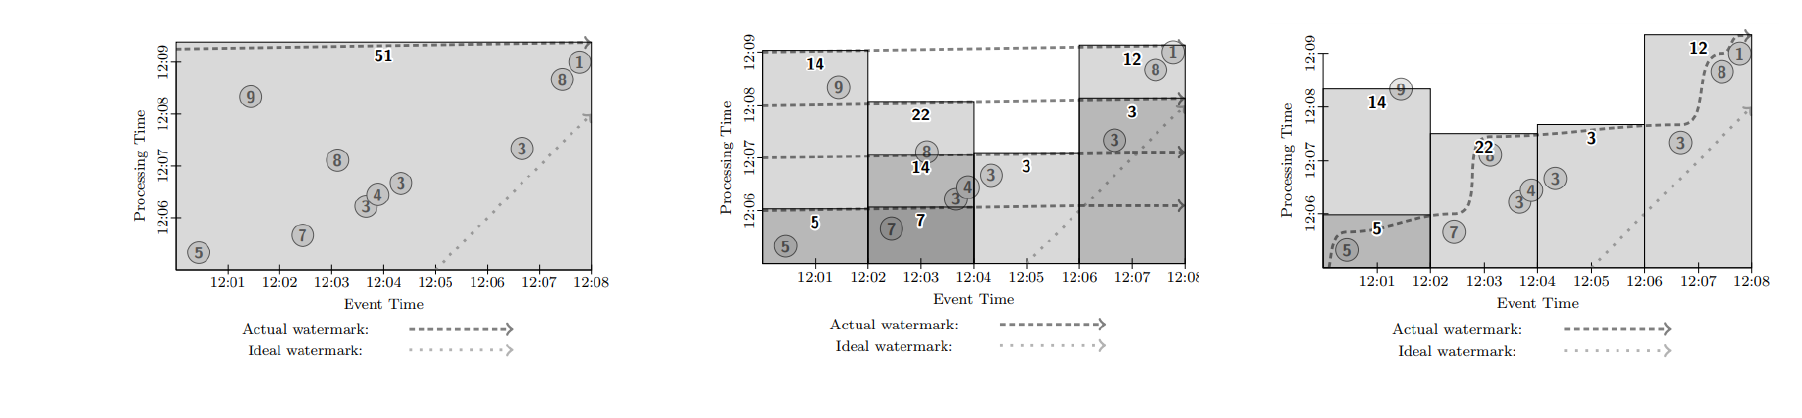
\includegraphics[width=0.9\textwidth]{pictures.png}\\
Fig. 2a, 2b, 2c
\end{center}
 
 Google Cloud Dataflow supports 3 different data processing styles. Here we explain how each of them works.
\begin{itemize}
    \item \textbf{Batching}: Google Dataflow just relies on MapReduce framework. The events must be all collected, then, they are sent together for  processing (Fig. 1a). Note that it is possible to split the data into smaller parts following the event-time period. However, the computation still happens after the collection of all the data. 
    \item \textbf{Mini-batch }: Mini-batch allows to process data at a lower latency compared with batch processing, but with a fair event correctness. The idea relies on applying windowing and triggering that can follow 2 possible approaches: 1) trigger at data (i.e. 2-events split); 2) trigger at period (i.e. 2-seconds split). In the case of Figure 2b, it is applied a trigger at period (1 minute event-time) and windowing at 2 minutes event-time, defining the instant after which the computation of the data collected will happen. The watermark jumps from the beginning of batch to end of time instantaneously. Event correctness is applied since a window can be kept open until more data comes in (for instance, event 9 in the first window).
    \item \textbf{Streaming}. Streaming relies on watermarks i.e. event signals that are sent heuristically that give information about when to close a window and process data. The goal of streaming-processing is to process data with the lowest latency possible. However, in case of late events, it is possible to consider 2 \textit{refinements} approaches: 1) discard the event (simple \textit{streaming}), 2) set an \textit{AllowedLateness} frame in which the windows can be kept open, as it happens in Fig. 2c with the window 12.00 to 12.02 (\textit{streaming + accumulation}). A window must of course be closed to avoid memory issues.
\end{itemize}

 

\end{enumerate}


\end{document}